\section{\label{sec3}\normalsize EXEMPLOS DE CÓDIGOS}
	
	\begin{lstlisting}
//Tipos numéricos:
a = 2;
b = 1;
f = 0.123;
teste = 2;
	
//Boolean	
j = false;
	
//String
frase = "Teste";
	
//Função
func helloWordl() {

  //Chamar um função
  printMessage("Testando, 1,2,3");
		
  //If-then-else
  if (a > 3) {
    b = 3*(1+2);
  } else {
    a = 1.3 - 9.456;
  }
		
  //Switch
  switch teste {
    case 1:
      t = u;
    case 2:
      a = 1 + 1;
    case 3:
      l = true;
      j = false;
      break;
  }
		
  //For
  for(y = 0; y < 41; y = y + 1) {
    int = 1;
    float = 0.123;
  }
		
  //While
  while (teste < 100) {
    p = -1 + 1 * 8;
    q = (1+1)*(-8);
  }
}
	
func printMessage(message) {
  print(message);
}

helloWorld();
	\end{lstlisting}	
	\newpage
	\begin{sidewaysfigure}
	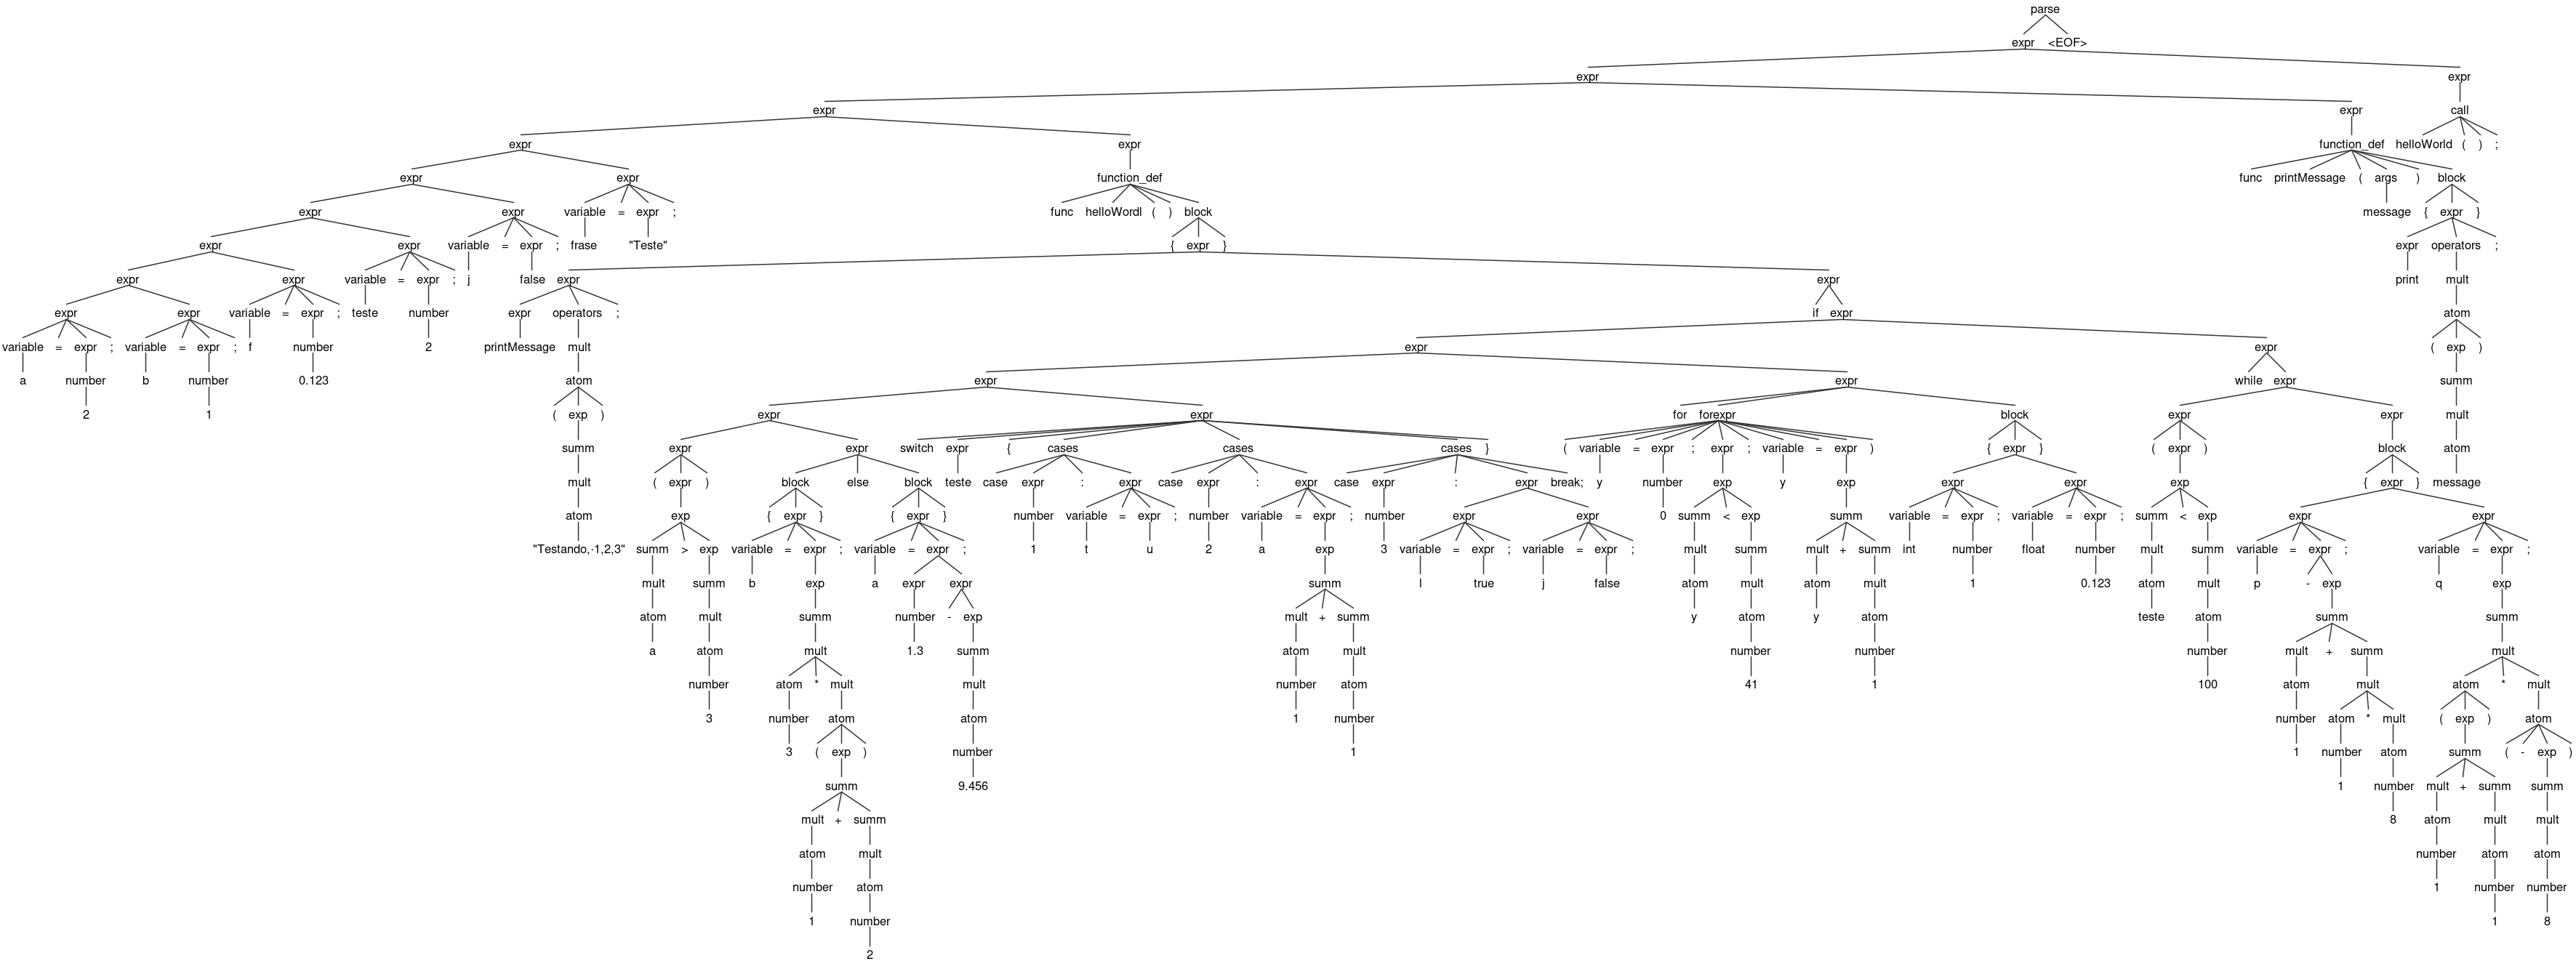
\includegraphics[width=1\textheight,height=0.8\textwidth]{01.png}
	\end{sidewaysfigure}